
\documentclass[withoutpreface,bwprint]{cumcmthesis} %去掉封面与编号页
\usepackage[final]{pdfpages}
\title{《软件需求工程 B》 大作业课题}
\tihao{A}
\baominghao{4321}
\schoolname{武汉理工大学}
\membera{小米}
\memberb{向左}
\memberc{哈哈}
\supervisor{老师}
\yearinput{2017}
\monthinput{08}
\dayinput{22}











\begin{document}
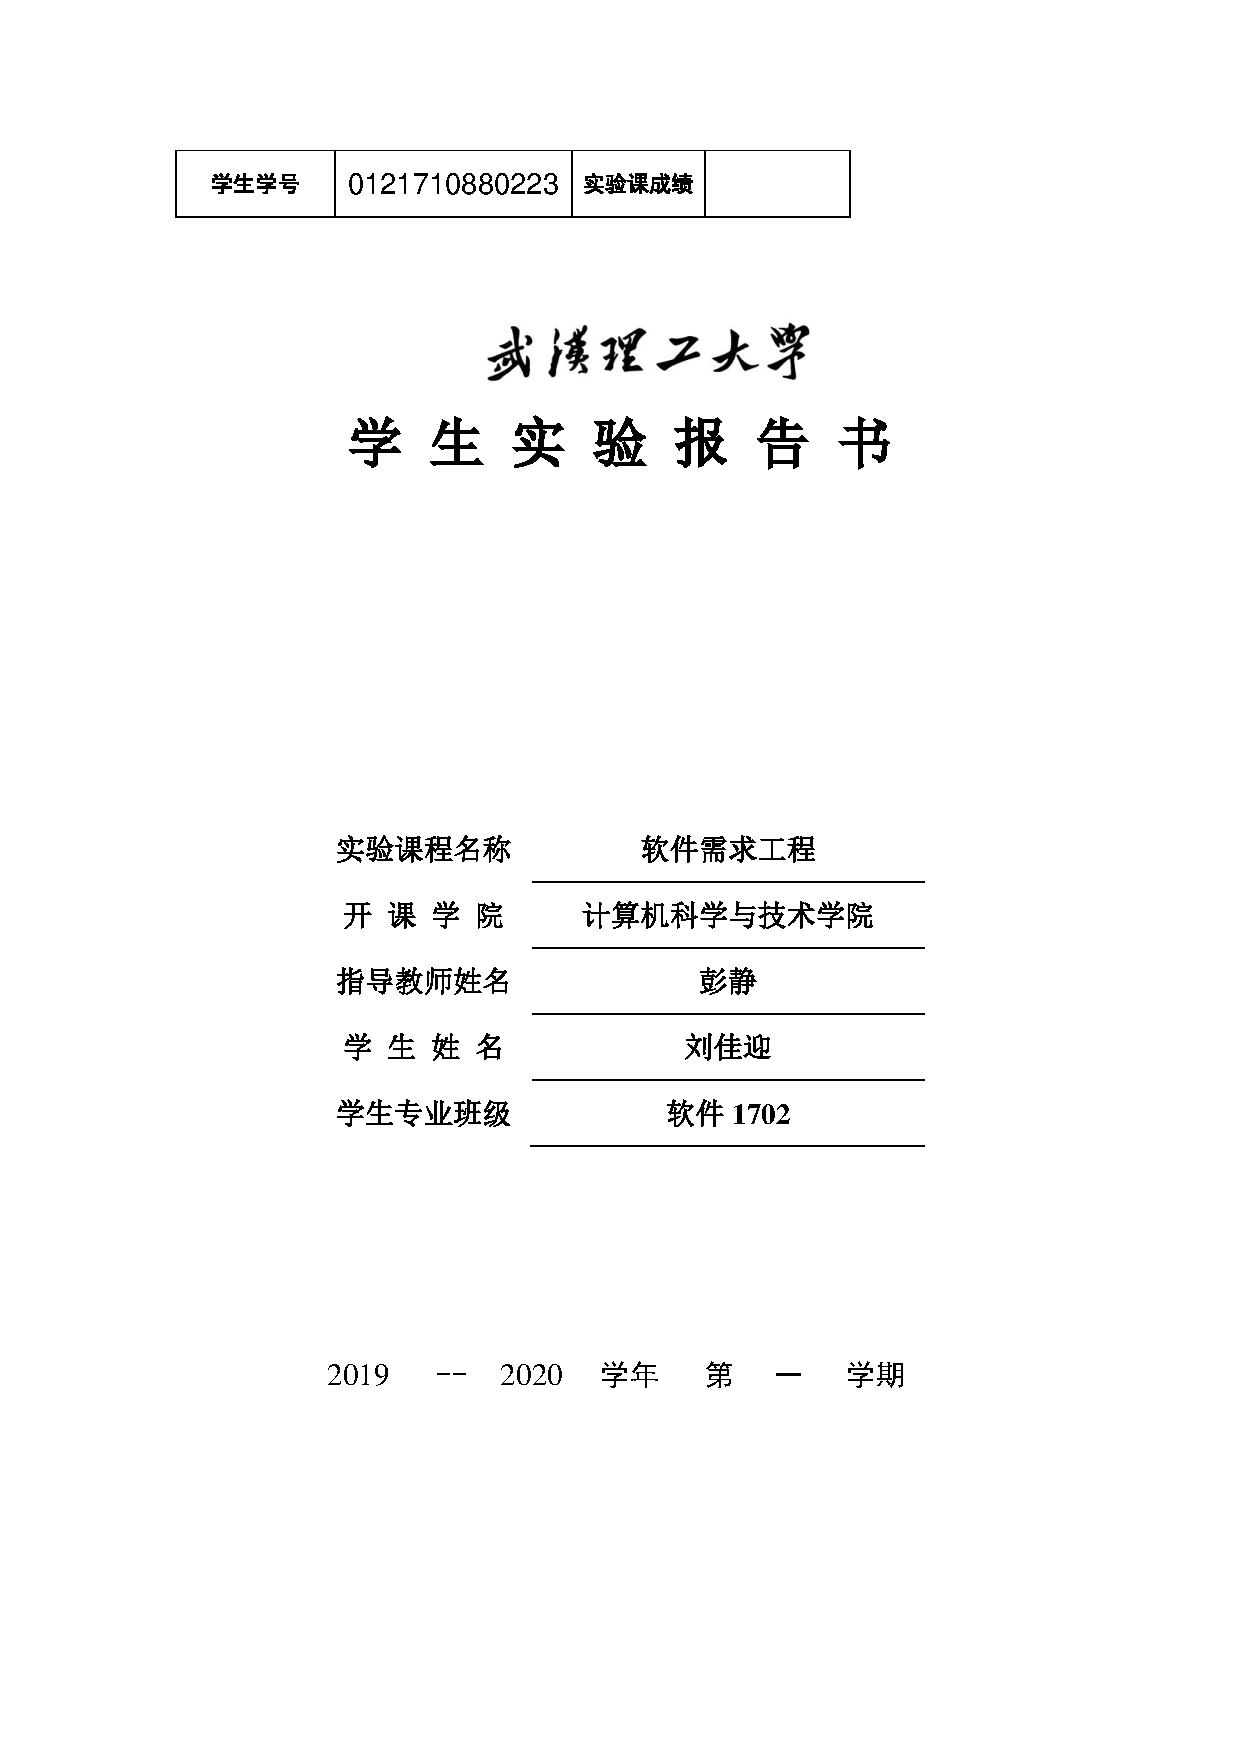
\includepdf{CoverOfExperimentalReport.pdf} 
\newpage
\section{美团评论分类实验报告}

\subsection{实验思路综述}

本次实验通过模拟美团Web端的Ajax请求,获得2万+的评论数据(中文评论+评分),并根据用户评分、中文评论构建二分类模型。

\subsection{爬取流程分析}

\begin{enumerate}
\item 分析Ajax请求$getPoiList$可以发现其主要由下面几个参数和一个token构成。通过解码token串,可以发现token也为固定参数经过编码后构成。
\begin{lstlisting}[language=python]
purl='https://wh.meituan.com/meishi/api/poi/getPoiList'
params={
    'cityName':'武汉',
    'cateId':0,
    'areaId':1006,
    'sort':'',
    'cityName': '武汉',
    'dinnerCountAttrId': '',
    'page': int(page_num),
    'uuid': puuid,
    'userId': 0,
    'platform': 1,
    'partner': 126,
    'originUrl': 'https://wh.meituan.com/meishi/b1006/',
    'riskLevel': 1,
    'optimusCode': 10,
    '_token': token
    }
page = requests.get(purl,params=params,headers=simulateChromeBrowserData)
\end{lstlisting}

模拟生成店铺POI的Ajax请求,获得店铺名称、Id、最大评论数。核心代码见附录A。
\item 根据美团评论数据的Ajax请求$getMerchantComment$可以发现主要有以下几个参数构成
\begin{lstlisting}[language=python]
purl='https://www.meituan.com/meishi/api/poi/getMerchantComment'
params = {
    'id' : shopID,
    'userId' : 0,
    'offset' : offSet*10,#偏移量,也是页码信息
    'pageSize' : 10,
    'sortType' : 1
    }
page = requests.get(purl,params=params,headers=simulateChromeBrowserData)
\end{lstlisting}
通过模拟该请求即可获得相关评论数据json包,为了提高运行速度,在获取评论信息的时候只保留中文字符,过滤掉字符数为空的评论数据。
\end{enumerate}

\subsection{分类流程分析}
本次实验使用了一些当下较火热的分类模型作为分类器,其中以LSTM模型为例介绍本次实验中的关键代码:
\begin{enumerate}
\item 首先读入数据格式,并对中文评论数据进行分词处理,并在迭代过程中去除停用词,
其实由于word2vec的算法依赖于上下文,且上下文有可能是停用词,因此可以不去停用词,但是比较结果发现去部分停用词后准确率提升了1\%左右。
\begin{lstlisting}[language=python]
def get_custom_stopwords(stop_words_file):
    with open(stop_words_file,encoding='gbk') as f:
        stopwords = f.read()
    stopwords_list = stopwords.split('\n')
    custom_stopwords_list = [i for i in stopwords_list]
    return custom_stopwords_list
def chinese_word_cut(mytext):
    cutted_com=[]
    stop_words_file = "/content/comment-analysis/stopwords/中文停用词库.txt"
    stopwords = get_custom_stopwords(stop_words_file)
    sentence_seged = jieba.cut(mytext)
    for word in sentence_seged:
        if word not in stopwords:
            cutted_com.append(word)
    return " ".join(cutted_com)
df['text'] = df.comment.apply(chinese_word_cut)
    \end{lstlisting}
\item 用分词器$Tokenizer$将句子中的词编码,因为每条评论长度不一,
而Keras在接受Input时需要序列长度一致,因此要使用$pad\_sequences()$将文本序列转化为经过填充以后的一个长度相同的新序列。
\begin{lstlisting}[language=python]
    tokenizer = Tokenizer(num_words=max_words)
    tokenizer.fit_on_texts(df.cutted)
    sequences = tokenizer.texts_to_sequences(df.cutted)
    data = pad_sequences(sequences, maxlen=maxlen)
    \end{lstlisting}
\item 将数据划分为训练集和验证集,采用考虑到爬取到的数据量不是很大,因此拟采用添加$embedding$嵌入层的方法来初始化模型参数,
因此使用gensim库中的word2vec模型将之前的训练集词编码转化为词向量形式并传递给$embedding$层。
由于数据量较少,模型最终
采用了AI-challenge的细粒度情感分析里面的中文语料库进行模型的初始化,效果相较提升了8\%左右。
\begin{lstlisting}[language=python]
zh_model = KeyedVectors.load_word2vec_format('zh.vec')
···
model.add(Embedding(max_words, embedding_dim))
    \end{lstlisting}

\item 接下来就是构建lstm模型的时候了,如下表第一层是嵌入层,共有300000个已经初始化好的参数
,加入LSTM模型并在其后面加入$Dropout$层防止过拟合,
最终用一个全连接层$(sigmoid)$作为二分类模型的输出。
\begin{table}[!htbp]
    \caption{LSTM模型各层情况}\label{tab:002} \centering
    \begin{tabular}{ccccc}
        \toprule[1.5pt]
        Layer (type)&Output Shape&Param \# \\
        \midrule[1pt]
        embedding\_1 (Embedding)   &   (None, None, 300)  &       300000   \\ 
        lstm\_1 (LSTM)          &      (None, 32)         &       42624          \\ 
        dropout\_1 (Dropout)    &      (None, 32)         &       0        \\ 
        dense\_1 (Dense)        &      (None, 1)          &       33 \\
        \bottomrule[1.5pt]
    \end{tabular}
\end{table}

关键代码:
\begin{lstlisting}[language=python]
    units = 32
    model = Sequential()
    model.add(Embedding(max_words, embedding_dim))
    model.add(LSTM(units))
    model.add(Dropout(rate=0.2))
    model.add(Dense(1, activation='sigmoid'))
    model.summary()
        \end{lstlisting}

\item 使用高效的 ADAM 优化算法,二分类损失函数binary\_crossentropy(多分类的损失函数categorical\_crossentropy)
训练模型。
\begin{lstlisting}[language=python]
model.compile( optimizer=Adam(),
        loss='binary_crossentropy',
        metrics=['acc'])
history = model.fit(X_train, y_train,
                    epochs=10,
                    batch_size=32,
                    validation_data=(X_valid, y_valid))
#模型持久化
model.save(mypath/"mymodel.h5")
        \end{lstlisting}

\item 利用WordCloud库构建词云,效果如图 8 所示:
\begin{figure}[H]
    \centering
    \includegraphics[width=0.8\textwidth]{boys_ciyun.jpg}
    \caption{词云}
\end{figure}

实现代码:
\begin{lstlisting}[language=python]
wc = WordCloud(font_path="上首方圆体.ttf",background_color="white", max_words=2900, mask=alice_mask,
stopwords=stopwords)
#生成词云
wc.generate(text)
# store to file
wc.to_file(path.join(mypath/"ml-bayes-demo/boys_ciyun.jpg"))
plt.imshow(wc, interpolation='bilinear')
plt.axis("off")
plt.figure()
plt.imshow(alice_mask, cmap=plt.cm.gray, interpolation='bilinear')
plt.axis("off")
plt.show()
\end{lstlisting}
\end{enumerate}

\subsection{实验结果分析}
使用LSTM模型训练/测试的准确率和交叉熵如图 9 所示,最终验证集准确率为97.05\%(训练数据量只有1W+,
利用现有语料库初始化模型参数对模型准确率提升较大)

\begin{figure}[H]
    \centering
    \begin{minipage}[c]{0.4\textwidth}
        \centering
        \includegraphics[height=0.18\textheight]{ac1.png}
        \subcaption{准确率}
    \end{minipage}
    \begin{minipage}[c]{0.5\textwidth}
        \centering
        \includegraphics[height=0.18\textheight]{ac2.png}
        \subcaption{交叉熵}
    \end{minipage}
    \caption{LSTM模型结果}
\end{figure}
此外还用$textCNN,charCNN,Bi-LSTM,Bi-LSTM + Attention,RCNN,adver$

\noindent$sarialLSTM,Transformer,ELMo,Bert$等模型进行了实验,
对于TensorFlow2.0以及相关模型的原理理解的不是很多,代码见仓库(https://github.com/lj
yslyc/comment-analysis)

\subsection{总结与展望}

这次实验学了学NLP相关的知识,从Kaggle和AI-challenge得到了很多启发。同时看了TensorFlow2.0的
文档感觉收获较多。接下来正好要做一个书籍推荐系统,应该也可以加上书摘分类的模块来强化推荐系统。


\newpage
%附录
\begin{appendices}


\section{爬取店铺POI}

\begin{lstlisting}[language=python]
def decode_token(token):
    # base64解码
    token_decode = base64.b64decode(token.encode())
    # 二进制解压
    token_string = zlib.decompress(token_decode)
    return token_string
def encode_token(POI):
    ##结合武汉地区POI编号字符串
    strPOI = "https://wh.meituan.com/meishi/"+str(POI)+"/"
    # 生成token
    ts = int(datetime.datetime.now().timestamp() * 1000)
    token_dict = {
        'rId': 100900,
        'ver': '1.0.6',
        'ts': ts,
        'cts': ts + 100 * 1000,
        'brVD': [767,234],
        'brR': [[1536,864],[1536,834],24,24],
        'bI': [strPOI,""],
        'mT': ["304,119","304,116","306,114","308,111"],
        'kT': [],
        'aT': [],
        'tT': [],
        'aM': '',
        'sign': "eJwdjT1OAzEQhe+SwqV/lmSTjeQCpUJCdBxgsCfZEWt7ZY9BOUIuQkfBpX"
    }
    # 二进制编码
    encode = str(token_dict).encode()
    # 二进制压缩
    compress = zlib.compress(encode)
    # base64编码
    b_encode = base64.b64encode(compress)
    # 转为字符串
    token = str(b_encode, encoding='utf-8')
    return token
token = encode_token("b1006")
def parse_POI_Shop_Json(shop_json):
    one_page_data = pd.DataFrame()
    if 'data'in shop_json:
        for eachShopInfo in shop_json.get('data').get('poiInfos'):
            shopId = eachShopInfo.get('poiId')
            shopName = eachShopInfo.get('title')
            allCommentNum = eachShopInfo.get('allCommentNum')
            one_page_data = one_page_data.append(pd.DataFrame({'shopId':[shopId],
                                    'shopName':[shopName],'allCommentNum':[allCommentNum]}))
    return one_page_data
 \end{lstlisting}

 \section{评论数据爬取}

\begin{lstlisting}[language=python]
def getShopPage(shopID,offSet):
    simulateChromeBrowserData = {
        'Accept':'*/*',
        'Accept-Encoding':'gzip, deflate',
        'Accept-Language':'zh-CN,zh;q=0.8',
        'Connection':'keep-alive',
        'Host':'sz.meituan.com',
        'Referer':'http://wh.meituan.com/meishi/',
        'Cookie': '_lxsdk_cuid=16212a00d8ec8-07cdb6596bad8e-178123e-1fa400-16212a00d8fc8; lat=22.780886;
                     lng=113.906362; client-id=34908f62-ea11-4211-b60a-f62c32288b2e; uuid=9be4f96971ac4c9cab4c.1520730903.1.0.0; webloc_geo=22.527181%2C113.938582%2Cwgs84; ci=30; _lxsdk=16212a1cddfc8-011369480302e7-178123e-1fa400-16212a1cddfc8; 
                     __mta=247430459.1520730902128.1520731016684.1520731025187.5; _lxsdk_s=16212a00d8f-c83-6e-376%7C%7C9',
        'User-Agent':'Mozilla/5.0 (Windows NT 10.0; Win64; x64) AppleWebKit/537.36 
                     (KHTML, like Gecko) Chrome/76.0.3809.100 Safari/537.36'
    }
    purl='https://www.meituan.com/meishi/api/poi/getMerchantComment'
    params = {
        'id' : shopID,
        'userId' : 0,
        'offset' : offSet*10,#偏移量,也是页码信息
        'pageSize' : 10,
        'sortType' : 1
    }
    page = requests.get(purl,params=params,headers=simulateChromeBrowserData)
    return page
def dataClean(comment):  #只保留中文
    pattern = re.compile(r'[^\u4e00-\u9fa5]')
    commentc = re.sub(pattern, '', comment)
    return commentc

def parse_POI_Shop_Json(shop_json):
    one_comment_data = pd.DataFrame()
    if 'data'in shop_json:
        for eachShopInfo in shop_json.get('data').get('comments'):
            Comment = dataClean(eachShopInfo.get('comment'))
            if not Comment:
                continue
            IsGreet = 1 if eachShopInfo.get('star')>= 30 else 0
            one_comment_data = one_comment_data.append(pd.DataFrame({'comment':[Comment],
                                                            'sentiment':[IsGreet]}))
    return one_comment_data
\end{lstlisting}





\end{appendices}

\end{document}
